\index{}\documentclass[a4paper, 11pt, fleqn, leqno ]{article}

%%%%%%%%%%%%%%%%%%%%%%%%%%%%%%%%%%%%%%%%%%%%%%%%%%%%%%%%%%%%%%%%%%%%%%%%%%%
%%%%%%%%%%%%%%%%%%%%%%% Preamble %%%%%%%%%%%%%%%%%%%%%%%%%%%%%%%%%%%%%%%%%%
%%%%%%%%%%%%%%%%%%%%%%%%%%%%%%%%%%%%%%%%%%%%%%%%%%%%%%%%%%%%%%%%%%%%%%%%%%%
%%%% General %%%%
\usepackage[left=25mm, right=25mm, top=20mm, bottom=20mm]{geometry}
\usepackage[ngerman, english]{babel}
\usepackage[utf8]{inputenc} %%% Check that document and editor are utf8 encoded!
\usepackage{bold-extra} %% Damit kann man Kapitälchen fett schreiben.
\usepackage{graphicx}
\usepackage[percent]{overpic} %%Damit lädt man Text über ein Bild.
\usepackage{setspace}
%\setlength{\parskip}{1ex} %% Abstand zwischen Absätzen
%\setlength{\parindent}{0pt} %% Länge des Einzugs bei Beginn eines Absatzes
\usepackage{tabularx} %% tables
\usepackage{hhline} %% Double line in tables
\usepackage{float} %% fix position of tables
\usepackage{paralist}
\usepackage{chngcntr}  %% Manage footnote count
\usepackage{color}
\usepackage{xcolor}
\usepackage{blindtext}
\usepackage[colorlinks]{hyperref} %% option colorlinks for colorful hyperrefs, for online version
%\usepackage[pdftex]{hyperref}   %% option pdftex for colorless hyperrefs, for printed version
%\clubpenalty = 10000 % Schusterjungen verhindern
%\widowpenalty = 10000 % Hurenkinder verhindern

%%%% Bibliography  %%%%
\usepackage{natbib} %% bibliography 
%\usepackage[sectionbib]{natbib} for references not starting a new page in document class report
\bibliographystyle{chicago} %% bibliography style
\usepackage[normalem]{ulem} %% z.B. zum Durchstreichen, Option [normalem] bewirkt, dass Journals u.ä. weiterhin kursiv dargestellt werden.
\setcitestyle{notesep={:}} %% saparates page numbers with colon in citations
\providecommand{\noopsort}[1]{} %% sort names with prefix such as von or van


%%%% Linguistics Packages %%%%
\usepackage{tree-dvips} %% draw arrows on trees
\usepackage{qtree}
\usepackage{stmaryrd, amsmath, amssymb}
\usepackage{linguex} %% linguistic examples
%\nosinglegloss %% Zeilenabstand zwischen Glossen wie im restlichen Text.
\usepackage{wasysym} %% symbols
\usepackage{marvosym} %% symbols
\usepackage{amsthm} %% math stuff?
\usepackage{dsfont} %% math symbols
\newtheorem{definition}{Definition}
%Repeat an example number
%begin new command example repetition
\makeatletter
\newif\if@repeated\@repeatedfalse
\newcounter{savedExNo}
\renewcommand{\NormalEx}{\ifExWarning 
     \PackageWarning{linguex}{Check example numbering (screwed up?), 
     check number of empty lines at end of examples.  
     Detected}\fi\ExWarningtrue
     \if@repeated
        \Exformat[\ref{\tmp@ref}]
        \setcounter{ExNo}{\value{savedExNo}}
        \global\@repeatedfalse
     \else
     \if@noftnote\refstepcounter{ExNo}%
        \Exformat[\ExLBr\Exarabic{ExNo}\ExRBr]%
     \else
         \refstepcounter{FnExNo}\Exformat[\FnExLBr\Exroman{FnExNo}\FnExRBr]%
     \fi
     \fi}
\newcommand{\exr}[1]{%
\@repeatedtrue
\setcounter{savedExNo}{\value{ExNo}}
\def\tmp@ref{#1}
\ex.}

\makeatother
%end new command
%%%%%%%%%%%%%%%%%%%%%%%%%%%%%%%%%%%%%%%%%%%%%%%%%%%%%%%%%%%%%%%%%%%%%%%%%%%
%%%%%%%%%%%%%%%%%%%%%%% End Preamble %%%%%%%%%%%%%%%%%%%%%%%%%%%%%%%%%%%%%%
%%%%%%%%%%%%%%%%%%%%%%%%%%%%%%%%%%%%%%%%%%%%%%%%%%%%%%%%%%%%%%%%%%%%%%%%%%%


\begin{document}
%%%% Document information %%%%
\definecolor{darkmidnightblue}{rgb}{0.0, 0.2, 0.4}  %define color for citations
\author{Swantje Tönnis}
\title{Results -- Pilot `QUD expectations'}
\hypersetup{
    pdftitle = {\@title},
    pdfauthor = {\@author},
    citecolor = {darkmidnightblue}, % change color of citations
    allbordercolors = {white},		% change color of frames
    linkcolor = {darkmidnightblue}, % change color of examples and contents
    urlcolor= {darkmidnightblue}	% change color of website links
}
\maketitle
\section{Baseline Qs}

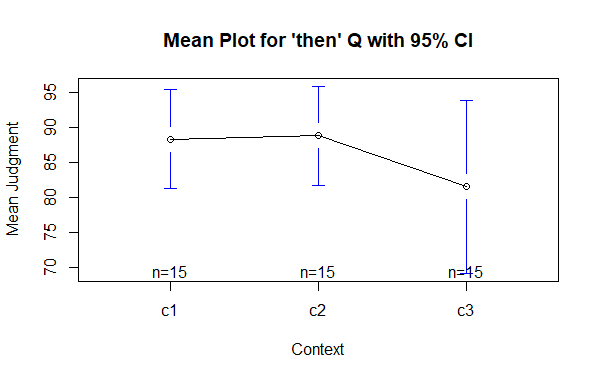
\includegraphics[width=0.9\textwidth]{means_thenQ.png}\\
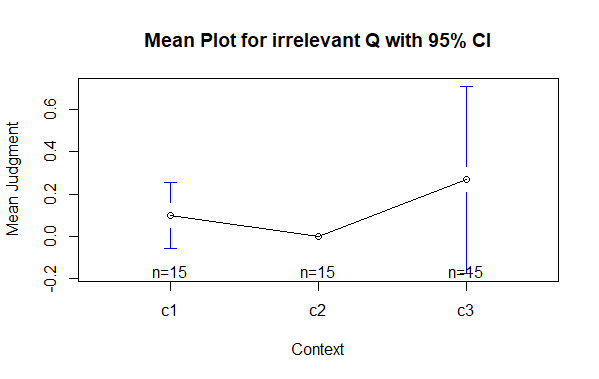
\includegraphics[width=0.9\textwidth]{means_irrelevantQ.png}

\section{PQs}\vspace{-2ex}
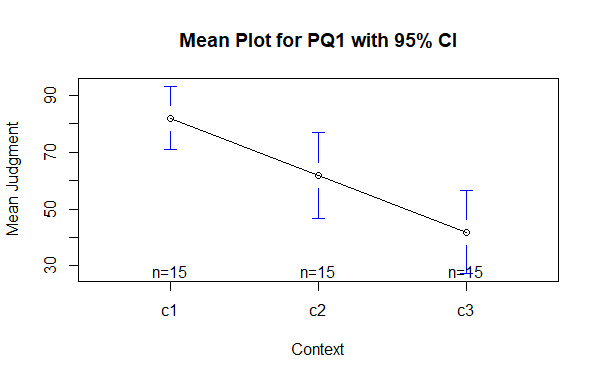
\includegraphics[width=0.8\textwidth]{means_PQ1.png}\\
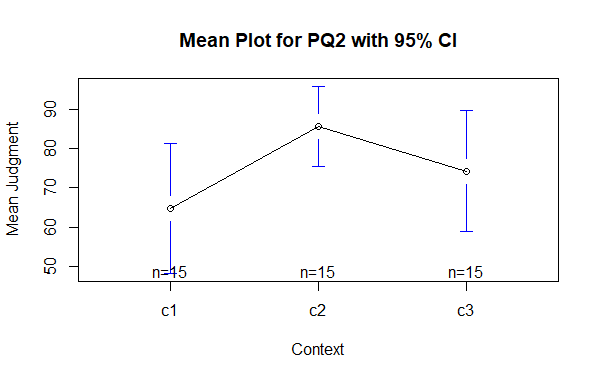
\includegraphics[width=0.8\textwidth]{means_PQ2.png}\\
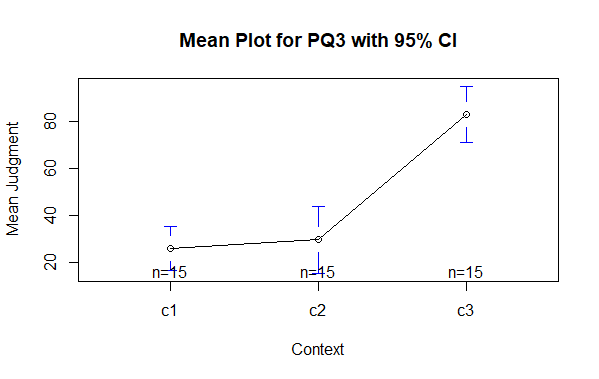
\includegraphics[width=0.8\textwidth]{means_PQ3.png}

\section{Comparison of all questions in a context}\vspace{-2ex}
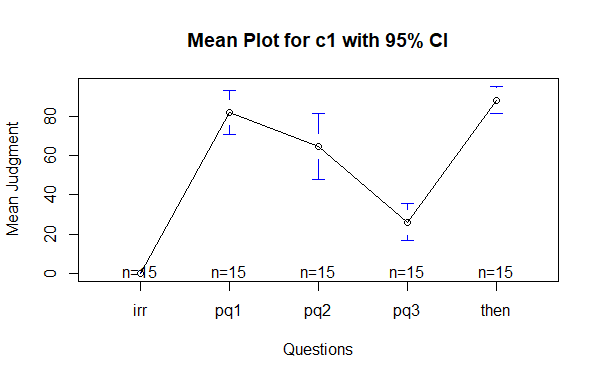
\includegraphics[width=0.8\textwidth]{means_c1.png}\\
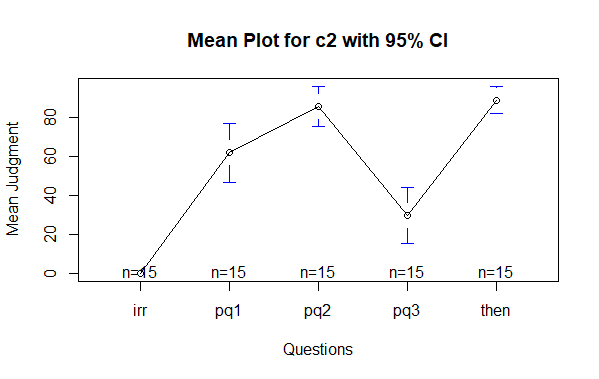
\includegraphics[width=0.8\textwidth]{means_c2.png}\\
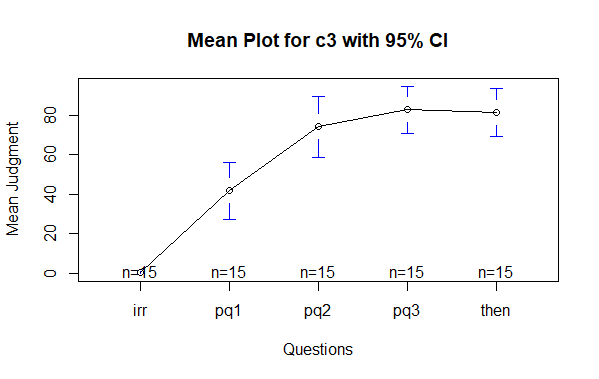
\includegraphics[width=0.8\textwidth]{means_c3.png}
\bibliography{mybib}
%\bibliography{C:/Arbeit/Literature/mybib}
\end{document}